\RequirePackage{ifpdf}
\ifpdf
   \documentclass[a4paper,11pt,pdftex,twoside]{scrartcl}
\else
   \documentclass[a4paper,11pt,dvips,twoside]{scrartcl}
\fi

% ------------------------------------------------------------------------------
% Include packages
% ------------------------------------------------------------------------------
\ifpdf
   \usepackage[pdftex]{color}
   \usepackage[final,pdftex]{graphicx} % Einbinden von Gaphiken, flexibler als package {graphics}
\else
   \usepackage[dvips]{color}
   \usepackage[final,dvips]{graphicx}
\fi
\usepackage[german]{babel}
\usepackage[T1]{fontenc}
\usepackage{caption}
\usepackage{url}
\usepackage{tabularx}
\usepackage{booktabs}
\usepackage{longtable}
\usepackage[table]{xcolor}
\usepackage{xspace}   % \xspace
\usepackage{float}
\usepackage{lscape}
\usepackage[left=2cm,right=2cm,top=1cm,bottom=1cm,includeheadfoot]{geometry}
\usepackage{rotating} 
\usepackage{url}


% PAGE LAYOUT
%\setlength{\topmargin}{-1cm}
%\setlength{\headheight}{0cm}
%\setlength{\headsep}{0cm}


%\setlength{\textheight}{\paperheight}
%\addtolength{\textheight}{-1in}

\setlength{\oddsidemargin}{0.1cm}
\setlength{\evensidemargin}{\oddsidemargin}
\setlength{\textwidth}{\paperwidth}
\addtolength{\textwidth}{-2in}
\addtolength{\textwidth}{-1.8\oddsidemargin}

% new commands
\newcommand{\superscript}[1]{\ensuremath{^{\textrm{#1}}}}
\newcommand{\subscript}[1]{\ensuremath{_{\textrm{#1}}}}

\renewcommand{\th}[0]{\superscript{th}}
\newcommand{\st}[0]{\superscript{st}}
\newcommand{\nd}[0]{\superscript{nd}}
\newcommand{\rd}[0]{\superscript{rd}}

\newcommand{\celsius}{$^{\circ}\mathrm{C}$\xspace}
\newcommand{\degree}{$^{\circ}$\xspace}

% Color defintions
\definecolor{gray1}{rgb}{0.95,0.95,0.95}
\definecolor{gray2}{rgb}{0.85,0.85,0.85}

%
\newcommand{\inspire}{\emph{Inspire St.Gallen\xspace}}

% ============================================================================
% Define Titlepage
% ============================================================================
%\subject{}
\title{Energie Modell (MAG)\\NDM200}
%\author{Conrad Dietschweiler}
\date{Datum: 10. Juni 2011 \\
Version: 0.1  (27. Juni 2011)}
%\publishers{\vspace{20mm}}  % Abused to separate title from abstract
\titlehead{
    \vspace{-15mm} 
    \hspace{-3mm}
    \begin{tabular}{lp{3cm}l}
        
\includegraphics[width=65mm]{Bilder/eth_logo} &&
        
\includegraphics[width=45mm]{Bilder/Inspire_Logo}\\
    \end{tabular}
    \vspace{10mm} 
    \hspace{0mm}

}
% ============================================================================

\begin{document}

% ----------------------------------------------------------------------------
% Make titlepage
% ----------------------------------------------------------------------------
\maketitle
\thispagestyle{empty} % No headers, no page numbers
% Include title picture
\begin{figure}[htbp]
\begin{center}
  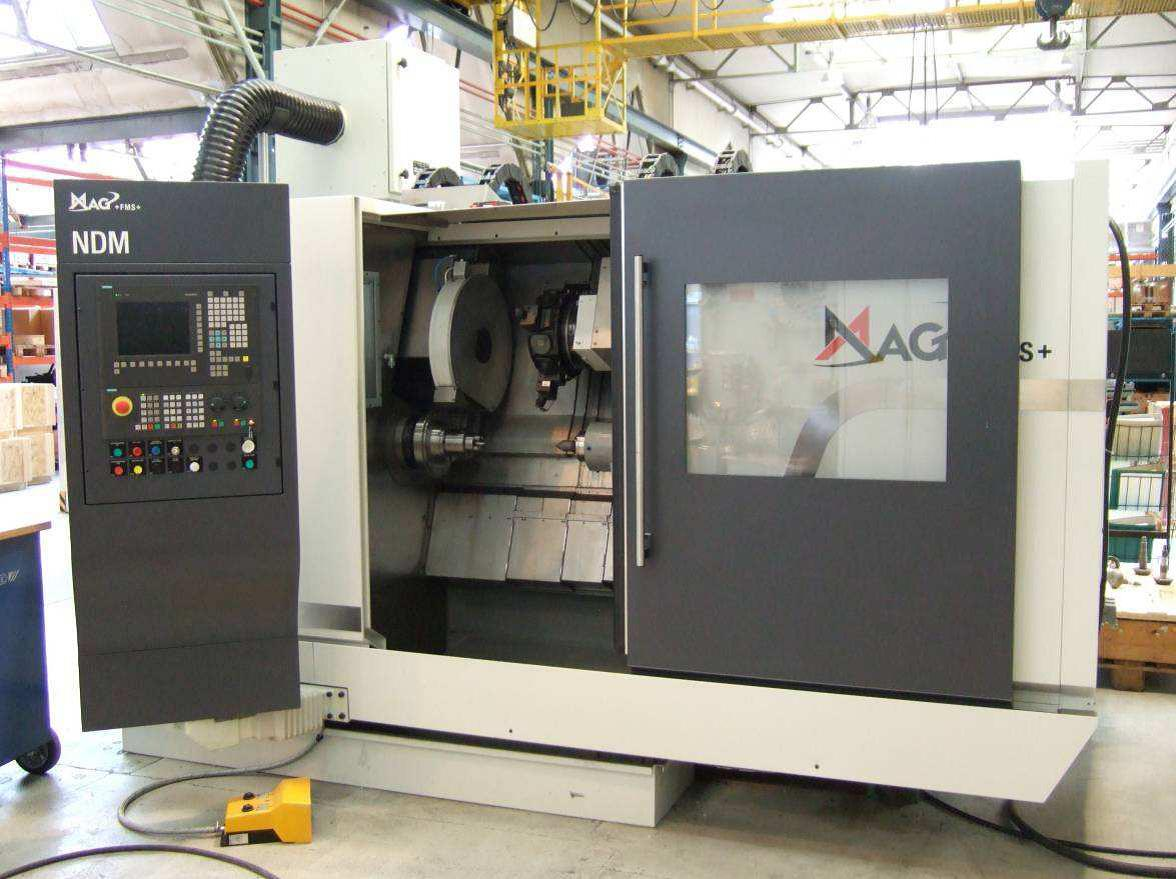
\includegraphics[width=0.7\columnwidth]{Bilder/NDM200.jpg}
  \caption*{NDM 200}
\end{center}
\end{figure}

\clearpage

\thispagestyle{empty} % No headers, no page numbers
\tableofcontents
\clearpage

%\pagestyle{plain} % No headers, just page numbers
\pagenumbering{arabic} % Roman numerals
\setcounter{page}{1}   % Start page numbering

% ----------------------------------------------------------------------------
% Einleitung
% ----------------------------------------------------------------------------
\section{Einleitung}



% ----------------------------------------------------------------------------
% Maschine
% ----------------------------------------------------------------------------
\section{Maschine}

\subsection{Beschreibung}

Die NDM 200 ist eine Drehmaschine. Bei dieser Messung wurde ein VDI-Teil ohne R\"usten gefr\"ast. 



\subsection{Systemgrenzen}

Die Systemgrenzen ziehen wir um die Maschine inklusiv K\"uhlaggregate. Wir
messen die zugef\"uhrte elektrische Leistung, die Druckluft- und den Stickstoffverbrauch. Tabelle \ref{tab:consumers_notmeasured}
listet nicht ber\"ucksichtigte Energiefl\"usse auf.

\paragraph{Ausnahme:}
Bei der Umrechung der gemessenen Druckluft in elektrische
Energie ber\"ucksichtigen wir den Wirkungsgrad eines durchschnittlichen
Kompressors. 


\pagebreak
\subsection{Gemessene Verbraucher}

Tabelle~\ref{tab:consumers} listet die gemessenen Energieverbraucher auf.

\begin{table}[H]
\caption{Gemessene Verbraucher}
\label{tab:consumers}
\rowcolors{1}{gray1}{gray2}
\begin{tabularx}{\textwidth}{llX}
  {\bf ID} & {\bf Name}            & {\bf Beschreibung} \\
  100 & Gesamteinspeisung          & Zuleitung aller elektrischen Verbraucher 400 V AC\\
  10  & Versorgung 24~V              &  E/A-Module, Bremsen, 24V-DC \\
  11  & Versorgung 230~V        & \\
  12  & E/R Modul        &  \\  
  13  &  \"Uberwachungsmodul   & \\
  20  & CNC              &  Gesamtleistung aller Achsen. Gemessen vor dem Umrichter, 400V-AC \\
  30  & Absaugungsvorrichtung              &  \\
  40  & Hydraulikpumpe              &  \\
  41  & Impulsschmierung             & \\
  50  & K\"uhlmittelpumpe Spindel        & Geschlossenes K\"uhlwassersystem f\"ur Spindel K\"uhlung \\
  51  & L\"ufter R\"uckk\"uhlung n1        & \\
  52  & L\"ufter R\"uckk\"uhlung n2        & \\
  60  & Schaltschrankk\"uhlung  links     &\\
  61  & Schaltschrankk\"uhlung rechts          & \\
  62  & E/R Modul L\"ufter            &\\
  70  & Druckluft                  & \\
\end{tabularx}
\end{table}


% ----------------------------------------------------------------------------
% Betriebszustaende
% ----------------------------------------------------------------------------
\section{Betriebszust\"ande und Prozesse}

Die gemessenen Betriebszust\"ande und Prozesse sind in Tabelle \ref{tab:states}
beschrieben.

\begin{table}[H]
\caption{Prozesse und Betriebszust\"ande}
\label{tab:states}
\rowcolors{1}{gray1}{gray2}
\begin{tabularx}{\textwidth}{llX}
  {\bf Nr.} &  {\bf Name}  & {\bf Beschreibung} \\
  1 & AUS      & Maschine spannungslos (Hauptschalter aus). \\
  2 & EIN      & Maschine AUS (Hauptschalter ist eingeschaltet, Steuerspannung nicht eingeschaltet, Aktoren spannungslos (Standby)). \\
  3 & ST-EIN-NOT      & Maschine EIN mit Nothalt (Steuerspannung eingeschaltet, Achsen nicht in Regelung. \\
  4 & ST-EIN      & Maschine EIN ohne Nothalt (Achsen in Regelung).\\
  5 & PR          & Maschine im Prozess (Achsen in Regelung, alle Einheiten laufen zyklisch je nach Prozessablauf). \\         
\end{tabularx}
\end{table}
\pagebreak


% ----------------------------------------------------------------------------
% Messungen
% ----------------------------------------------------------------------------

\section{Messungen}

\subsection{\"Uberblick}
Tabelle \ref{tab:measurements} listet die Messungen auf.


\begin{table}[H]
\begin{center}
\caption{Messungen}
\label{tab:measurements}
\rowcolors{1}{gray1}{gray2}
%\begin{tabularx}{\textwidth}{llllllll}
\begin{tabular}{lrrrrrrrrr}
  {\bf Name} & {\bf Zustand}& {\bf Beschreibung}&{\bf Zeit}\\
  M03	 & PR   	   &      VDI-Teil& 12:50-13:06\\
\end{tabular}
\end{center}
\end{table}



\subsection{\"Uberblick der mittleren Leistungen}

Abbildung \ref{fig:meas_overview} gibt einen \"Uberblick \"uber die mittleren
Leistungen der Verbraucher von allen Messungen. Tabelle \ref{tab:meas_power}
enth\"alt dieselbe Information.

\begin{figure}[H]
\begin{center}
  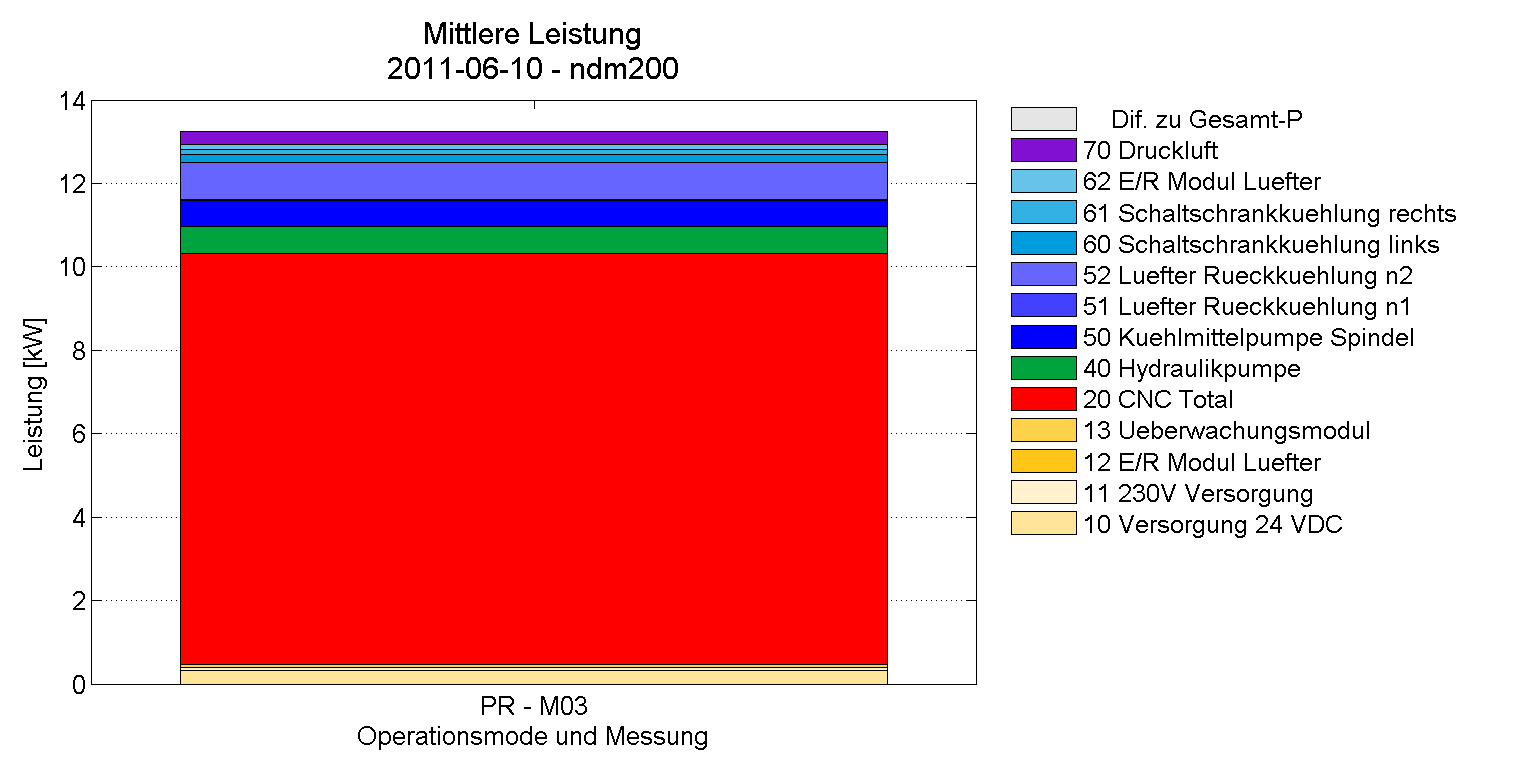
\includegraphics[width=\columnwidth]{figures/2011-06-10_ndm200_M031_cbar.png}
  \caption{\"Uberblick \"uber die mittlere Leistung.}
  \label{fig:meas_overview}
\end{center}
\end{figure}




% Tabelle der mittleren Leistung 
%\begin{landscape}


% Mean power table
\begin{table}[H]
\begin{center}
\caption{Mittlere Leistung in kW}
\label{tab:meas_power}
\begin{tabular}{lr}
 {\bf Verbraucher}  & {\bf M03} \\
  & kW  \\
\hline
 230V Versorgung   & 0.07  \\
 Versorgung 24 VDC   & 0.33  \\
 E/R Modul   & 0.00  \\
 Ueberwachungsmodul   & 0.07  \\
 CNC Total   & 9.86   \\
 Absaugungvorrichtung   & 0.00  \\
 Hydraulikpumpe   & 0.64  \\
 Kuehlmittelpumpe Spindel   & 0.61  \\
 Luefter Rueckkuehlung n1   & 0.04  \\
 Luefter Rueckkuehlung n2   & 0.87  \\
  Schaltschrankkuehlung links   & 0.21  \\
 Schaltschrankkuehlung rechts   & 0.11  \\
 E/R Modul Luefter   & 0.12  \\
\hline
Total Verbruacher (ohne DL)&12.02\\
 Einspeisung 400 VAC   & 11.94  \\
\hline
Differenz&-0.08\\
\hline
 Druckluft   & 0.30   \\
\hline
Total ( inkl. DL)&12.24\\
\hline
\end{tabular}
\end{center}
\end{table}
\pagebreak



\subsection{Messung M03: PR (VDI-Teil)}

\begin{figure}[H]
\begin{center}
  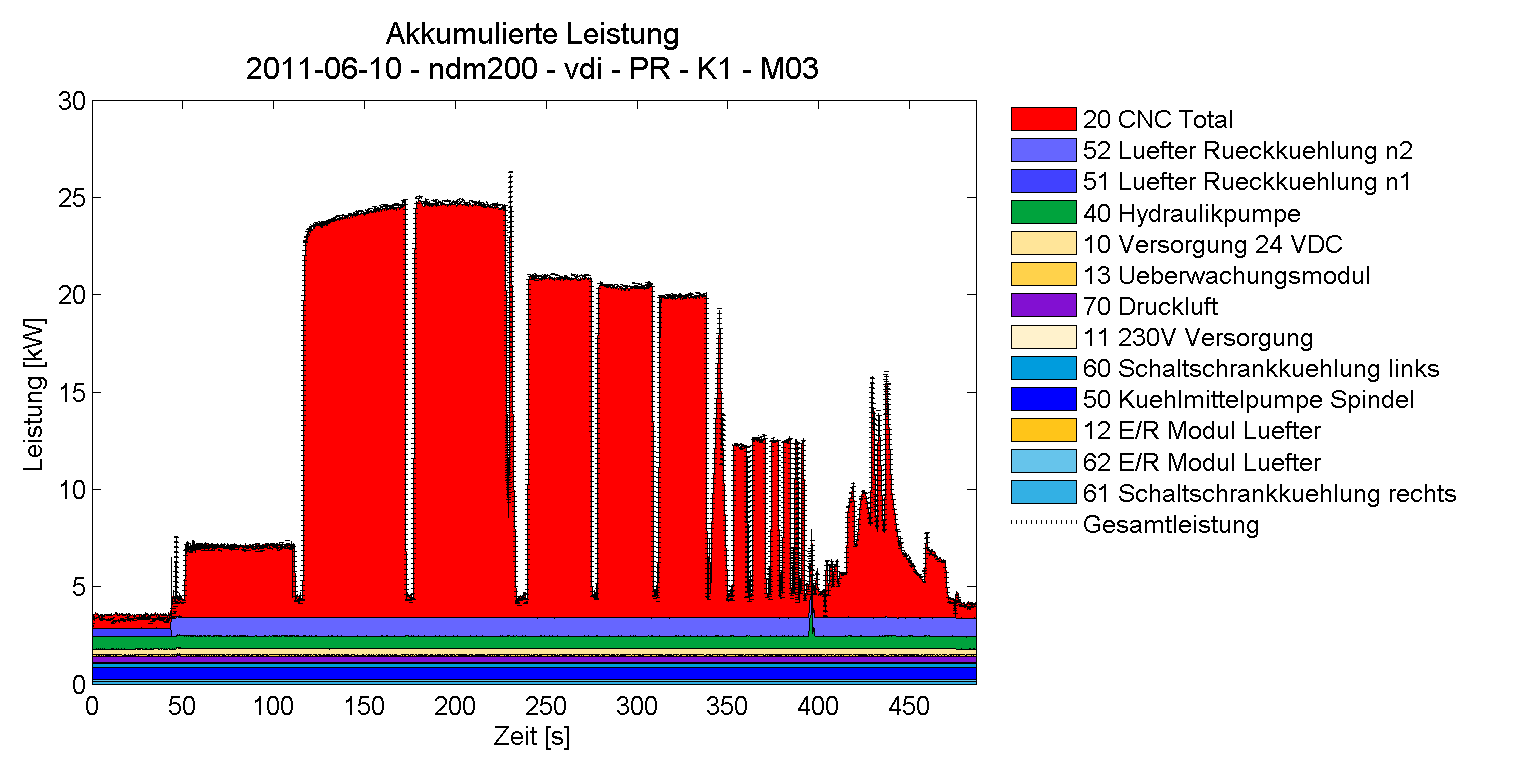
\includegraphics[width=\columnwidth]{figures/2011-06-10_ndm200_vdi_PR_K1_M031_area.png}
  \caption{Messung M03: Zeitverlauf der Leistungen.}
  \label{fig:M03_area}
\end{center}
\end{figure}

\begin{figure}[H]
\begin{center}
  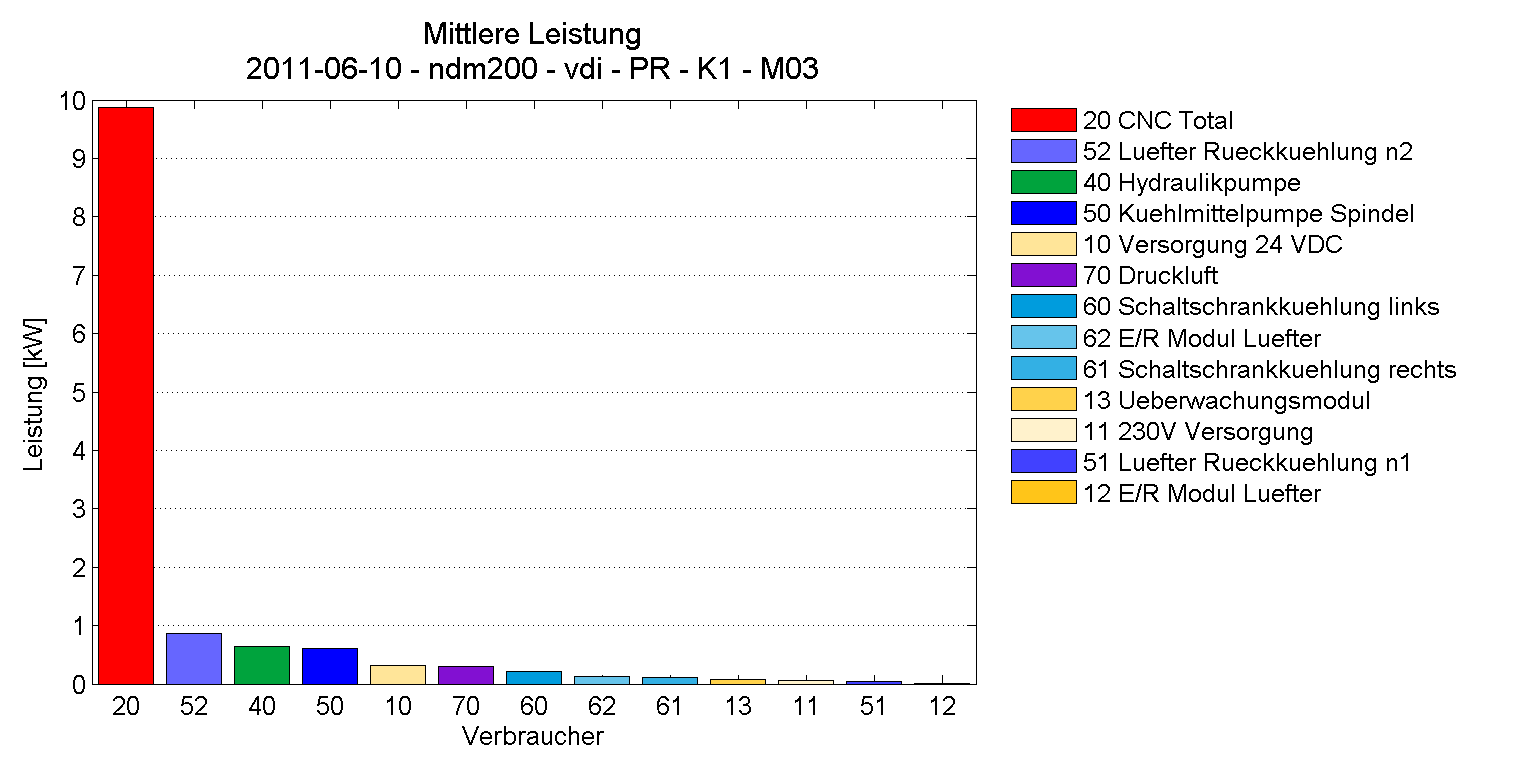
\includegraphics[width=\columnwidth]{figures/2011-06-10_ndm200_vdi_PR_K1_M031_bar.png}
  \caption{Messung M03: Mittlere Leistung der einzelnen Verbraucher.}
  \label{fig:M03_bar}
\end{center}
\end{figure}
\pagebreak




\subsection{Leistung der CNC Komponenten f\"ur  Messung M03}

% Tabelle der mittleren Leistung 
%\begin{landscape}


% Mean power table
\begin{table}[H]
\begin{center}
\caption{Mittlere Leistung in kW}
\label{tab:meas_power}
\begin{tabular}{lr}
  {\bf Verbraucher}  & {\bf M03} \\
  & kW  \\
\hline
 CNC Total   & 10.41\\
 C1   & 6.47  \\
 W   & 0.34  \\
 X1   & 0.00  \\
 X2   & 0.00  \\
 Z1   & 0.00  \\
 Z2   & 0.01  \\
\hline
 Total  & 17.22  \\
\hline
\end{tabular}
\end{center}
\end{table}



\begin{figure}[H]
\begin{center}
  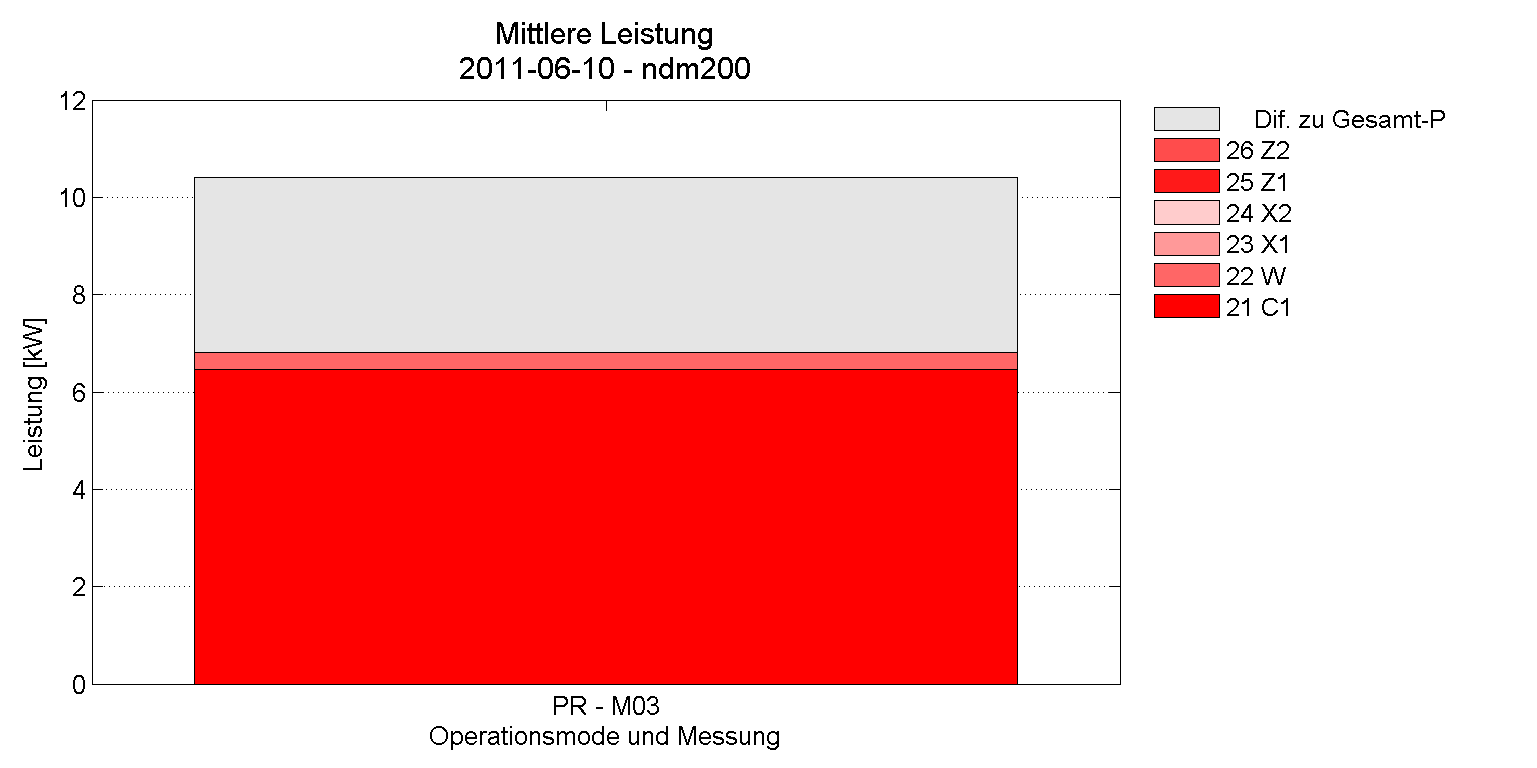
\includegraphics[width=\columnwidth]{figures/cnc/2011-06-10_ndm200_M03_cbar.png}
  \caption{Messung M03: Temperatur von NDM Komponenten.}
  \label{fig:M04_area}
\end{center}
\end{figure}
\pagebreak

\begin{figure}[H]
\begin{center}
  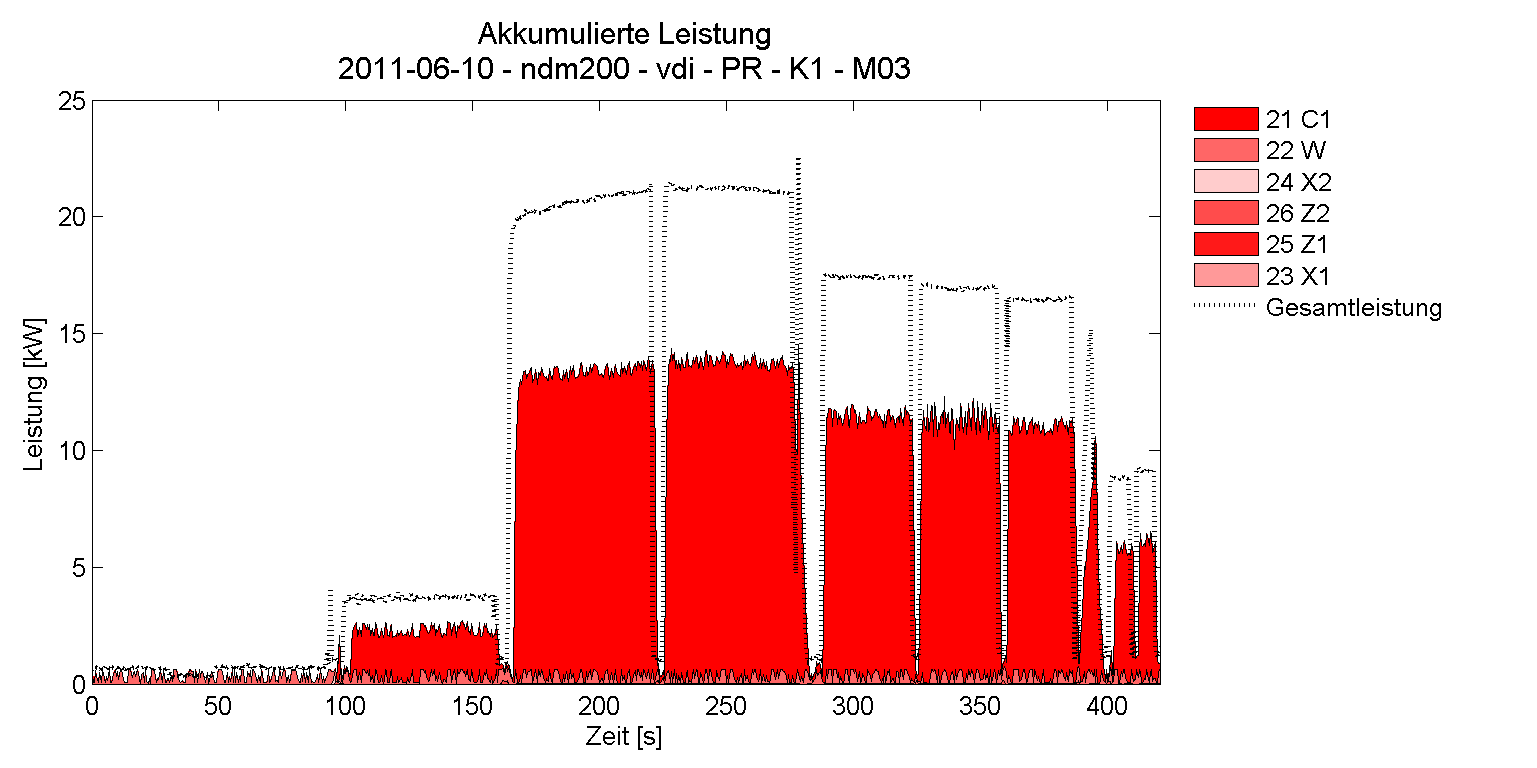
\includegraphics[width=\columnwidth]{figures/cnc/2011-06-10_ndm200_vdi_PR_K1_M03_area.png}
  \caption{Messung M03: Mittlere Leistung der einzelnen Verbraucher.}
  \label{fig:M03_bar}
\end{center}
\end{figure}


\begin{figure}[H]
\begin{center}
  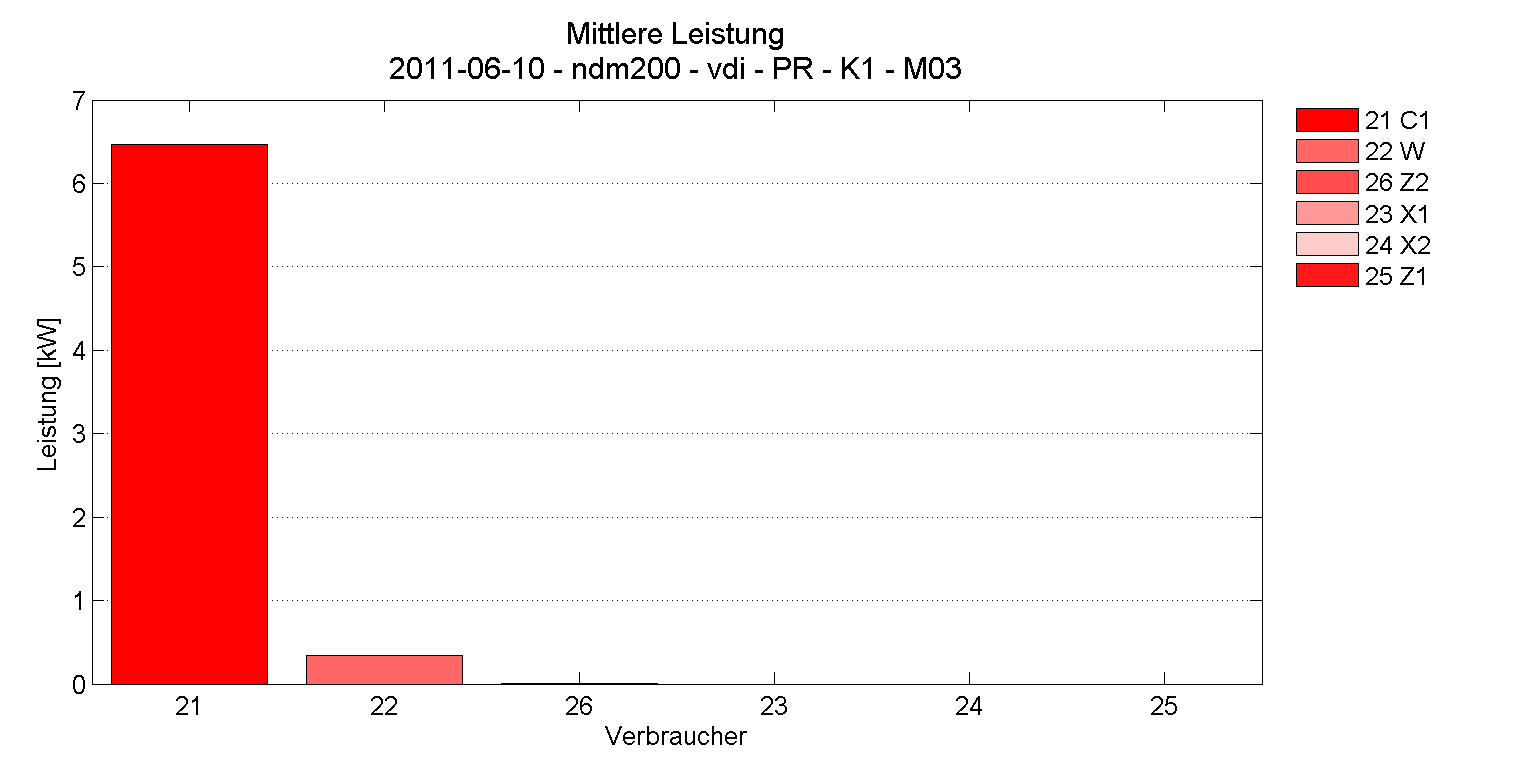
\includegraphics[width=\columnwidth]{figures/cnc/2011-06-10_ndm200_vdi_PR_K1_M03_bar.png}
  \caption{Messung M03: Mittlere Leistung der einzelnen Verbraucher.}
  \label{fig:M03_bar}
\end{center}
\end{figure}



\begin{figure}[H]
\begin{center}
  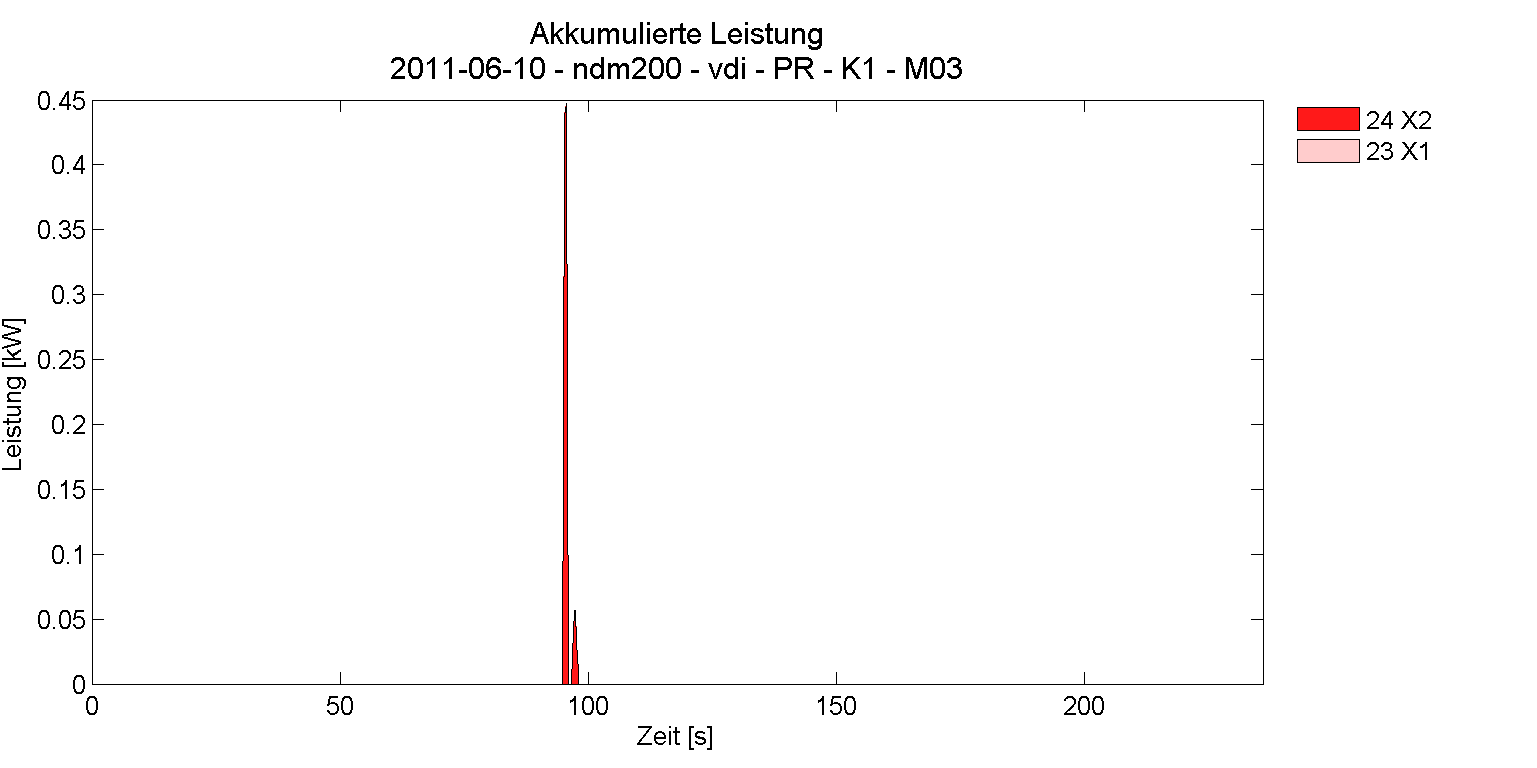
\includegraphics[width=\columnwidth]{figures/cnc/2011-06-10_ndm200_vdi_PR_K1_M03_area1.png}
  \caption{Messung M03: Temperatur von NDM Komponenten.}
  \label{fig:M04_area}
\end{center}
\end{figure}



\subsection{Temperatur von NDM Komponenten f\"ur  Messung M03}

\begin{figure}[H]
\begin{center}
  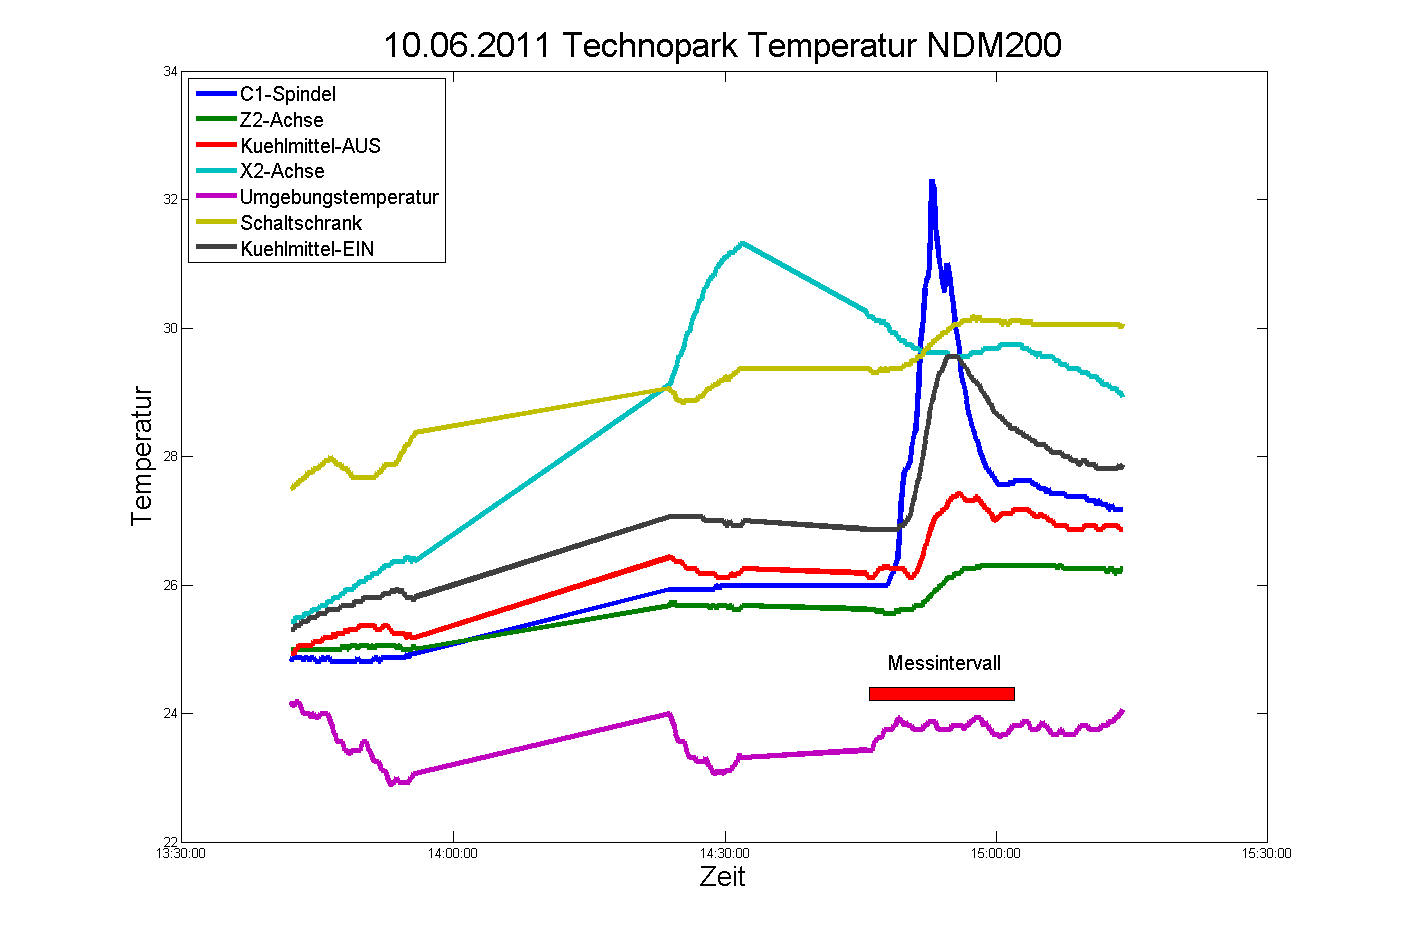
\includegraphics[width=\columnwidth]{figures/TemperaturNDM200.png}
  \caption{Messung M03: Temperatur von NDM Komponenten.}
  \label{fig:M04_area}
\end{center}
\end{figure}

\pagebreak





\appendix
% ----------------------------------------------------------------------------
% Fotos
% ----------------------------------------------------------------------------
%\section{Fotos}

% ----------------------------------------------------------------------------
% Literatur
% ----------------------------------------------------------------------------
\bibliographystyle{plain}  % alphabetic
\addcontentsline{toc}{section}{Literatur}

\begin{thebibliography}{1}


\bibitem{compair}
Bayrisches~Landesamt f\"ur Umweltschutz.
\newblock {Effiziente Druckluftsysteme}.
Augsburg 2004.


\end{thebibliography}



\end{document}